\documentclass[10pt,a4paper]{article}

\usepackage[utf8]{inputenc}
\usepackage{amsmath,amssymb,amsthm}
\usepackage{graphicx}
\graphicspath{{../QNet_Sim/results/experiments/figures/}}
\usepackage{hyperref}
\usepackage{booktabs}
\emergencystretch=1em
\usepackage[margin=1in]{geometry}
\usepackage{float}
\usepackage{xcolor}
\usepackage{fancyhdr}
\usepackage{titlesec}

\titleformat{\section}{\Large\bfseries}{\thesection}{1em}{}
\titleformat{\subsection}{\large\bfseries}{\thesubsection}{1em}{}
\titleformat{\subsubsection}{\normalsize\bfseries}{\thesubsubsection}{1em}{}

\newtheorem{definition}{Definition}[section]
\newtheorem{lemma}{Lemma}[section]
\newtheorem{proposition}{Proposition}[section]

\pagestyle{fancy}
\fancyhf{}
\fancyhead[L]{\small QiOpt4QNet -- Technical Report}
\fancyhead[R]{\small \today}
\fancyfoot[C]{\thepage}

\newcommand{\E}{\mathbb{E}}
\newcommand{\R}{\mathbb{R}}
\newcommand{\N}{\mathbb{N}}
\newcommand{\Z}{\mathbb{Z}}
\renewcommand{\H}{\mathcal{H}}
\newcommand{\tr}{\operatorname{tr}}
\newcommand{\diag}{\operatorname{diag}}
\newcommand{\argmin}{\operatorname{argmin}}
\newcommand{\argmax}{\operatorname{argmax}}

\begin{document}

\title{\textbf{Quantum-Inspired Optimization for Entanglement Routing\\
in Quantum Networks: A Technical Report\\
\large Full Mathematical Derivations, Solver Architectures,
and Experimental Analysis}}

\author{Arnav Kapoor\\
QiOpt4QNet Project\\
\url{https://github.com/arnavk23/QiOpt4QNet-Simulator}}

\maketitle

\tableofcontents
\newpage

%%%%%%%%%%%%%%%%%%%%%%%%%%%%%%%%%%%%%%%%%%%%%%%%%%%%%%%%%%%%%%%%%%%%%%
\section{Introduction and Motivation}
\label{sec:intro}
%%%%%%%%%%%%%%%%%%%%%%%%%%%%%%%%%%%%%%%%%%%%%%%%%%%%%%%%%%%%%%%%%%%%%%

Quantum networks distribute entanglement---the Bell-state correlations
$|\Phi^+\rangle = (|00\rangle + |11\rangle)/\sqrt{2}$---between distant
nodes.  Unlike classical networks, where a bit is a robust two-state
system, entanglement is a fragile resource that decays exponentially
with time (T1/T2 decoherence) and must be continuously regenerated via
probabilistic processes (entanglement swapping with success probability
$p_{\text{swap}} \ll 1$, BBPSSW purification rounds).

The core optimization problem is: given a set of concurrent
entanglement requests $\mathcal{R} = \{r_1, \dots, r_M\}$ between
source--destination pairs $(s_r, d_r)$ on a network graph
$G = (V, E)$, select for each request a path $p_r$ and purification
schedule $q_r$ (a \emph{bundle}) that maximizes end-to-end fidelity
while respecting edge and memory capacities.  This is a constrained
combinatorial optimization problem in $\mathcal{O}(|\mathcal{R}|^2)$
decision variables, which we formulate as a Quadratic Unconstrained
Binary Optimization (QUBO) problem and solve with three
quantum-inspired solvers.

This report provides a complete mathematical treatment of:
\begin{itemize}
  \item The quantum network model (Sec.~\ref{sec:model})
  \item The QUBO Hamiltonian with all penalty and physical terms
    (Sec.~\ref{sec:hamiltonian})
  \item Three solver architectures---Metropolis annealer,
    tensor-network (MPS) compressor, and streaming annealer
    (Sec.~\ref{sec:solvers})
  \item A comprehensive experimental benchmark with interpretation
    (Sec.~\ref{sec:results})
  \item A cross-domain comparison of QKD routing and entanglement
    routing assumptions (Sec.~\ref{sec:discussion})
\end{itemize}

The codebase is fully open source at
\url{https://github.com/arnavk23/QiOpt4QNet-Simulator} and all results
in this report are reproducible via \path{src/experiments/experiment\_suite.py}.

%%%%%%%%%%%%%%%%%%%%%%%%%%%%%%%%%%%%%%%%%%%%%%%%%%%%%%%%%%%%%%%%%%%%%%
\section{Quantum Network Model}
\label{sec:model}
%%%%%%%%%%%%%%%%%%%%%%%%%%%%%%%%%%%%%%%%%%%%%%%%%%%%%%%%%%%%%%%%%%%%%%

\subsection{Network Graph}

The quantum network is an undirected graph $G = (V, E)$ where each
edge $e = (u,v) \in E$ represents a fiber link between quantum
repeater nodes.  Each edge has:
\begin{itemize}
  \item Capacity $C_e \in \N$: maximum Bell pairs that can be
    simultaneously stored or in-flight per time epoch.
  \item Latency $\ell_e \in \R^+$: one-way propagation delay plus
    processing time.
  \item Raw fidelity $F_e^{(0)} \in [0,1]$: fidelity of the
    elementary Bell pair generated on link $e$ before purification.
\end{itemize}

Each node $v \in V$ has memory capacity $M_v^{\max} \in \N$,
representing the number of qubit slots available for storage.

\subsection{Entanglement Swapping and Purification}

Entanglement swapping at a repeater node consumes two Bell pairs
(one on each incident edge) and produces a new Bell pair connecting
the outer nodes, with a success probability
\begin{equation}
  p_{\text{swap}} = \frac{1}{2}
\end{equation}
for a Bell-state measurement in the standard basis.

BBPSSW purification~\cite{bennett1996purification} improves fidelity
at the cost of consuming additional Bell pairs.  Each round $q$ of
purification on a link of fidelity $F$ updates the fidelity as:
\begin{equation}
  F' = \frac{F^2 + (1-F)^2/3}{F^2 + 2F(1-F)/3 + 5(1-F)^2/9},
\end{equation}
where the denominator is the success probability of the purification
round.  After $q$ rounds, the end-to-end fidelity for a path of
$L$ links is approximately
\begin{equation}
  F_{\text{e2e}} \approx \prod_{e \in p} F_e^{(q_e)},
\end{equation}
assuming that entanglement swapping errors are dominated by the input
fidelity.

\subsection{Bundle Structure}

A \emph{bundle} $b$ for request $r$ is defined by:
\begin{itemize}
  \item A path $p_b = (v_0, v_1, \dots, v_{L+1})$ connecting
    $s_r = v_0$ to $d_r = v_{L+1}$.
  \item A purification profile $q_b = (q_1, \dots, q_L)$ specifying
    purification rounds per link.
  \item Success probability
    $p_{\text{succ}}^{(b)} = p_{\text{swap}}^{L} \cdot \prod_{e}
    p_{\text{purif}}(q_e)$.
  \item End-to-end fidelity $F^{(b)}$ after all swaps and
    purification.
  \item Latency $\ell^{(b)} = \sum_{e \in p_b} \ell_e$.
  \item Edge demands $d_{r,b}^e$: Bell pairs consumed on edge $e$.
  \item Memory demands $m_{r,b}^v$: qubit slots occupied at node $v$.
\end{itemize}

The \emph{utility} of selecting bundle $b$ for request $r$ is:
\begin{equation}
  u_{r,b} = w_r \cdot p_{\text{succ}}^{(b)}
    \cdot \bigl[1 + \beta \cdot \max(0, F^{(b)} - F_{\min})\bigr]
    - \lambda_\ell \cdot \ell^{(b)} - \lambda_c \cdot
    \text{cost}^{(b)},
\label{eq:utility}
\end{equation}
where:
\begin{itemize}
  \item $w_r$ is the request weight (priority),
  \item $F_{\min}$ is the minimum acceptable fidelity,
  \item $\beta$ is the marginal reward for exceeding $F_{\min}$,
  \item $\lambda_\ell$ penalizes latency,
  \item $\lambda_c$ penalizes resource cost (Bell pair consumption).
\end{itemize}

%%%%%%%%%%%%%%%%%%%%%%%%%%%%%%%%%%%%%%%%%%%%%%%%%%%%%%%%%%%%%%%%%%%%%%
\section{Hamiltonian Formulation}
\label{sec:hamiltonian}
%%%%%%%%%%%%%%%%%%%%%%%%%%%%%%%%%%%%%%%%%%%%%%%%%%%%%%%%%%%%%%%%%%%%%%

We formulate the entanglement routing problem as the minimization of
an energy function $\H : \{0,1\}^N \to \R$, where each binary variable
$x_{r,b} \in \{0,1\}$ indicates whether bundle $b$ is selected for
request $r$.  The total number of variables is
$N = \sum_{r=1}^M |B_r|$, where $B_r$ is the set of candidate
bundles for request $r$.

\subsection{Standard Penalty-Based QUBO}
\label{sec:standard-qubo}

The base Hamiltonian comprises four terms:

\subsubsection{Utility Term}
The total utility of a configuration is additive over selected bundles:
\begin{equation}
  \H_{\text{util}} = -\sum_{r=1}^M \sum_{b \in B_r} u_{r,b} \, x_{r,b}.
\end{equation}
Minimizing $\H_{\text{util}}$ maximizes the aggregate utility.

\subsubsection{One-Per-Request Constraint}
Exactly one bundle must be selected per request.  This is encoded as:
\begin{equation}
  \H_{\text{one-per-req}} = A \sum_{r=1}^M
    \Bigl(\sum_{b \in B_r} x_{r,b} - 1\Bigr)^2,
\end{equation}
where $A > 0$ is a penalty coefficient.  Expanding the square:
\begin{equation}
  \H_{\text{one-per-req}} = A \sum_r \Bigl(
    \sum_b x_{r,b}^2 - 2\sum_b x_{r,b} + 1\Bigr).
\end{equation}
Since $x_{r,b}^2 = x_{r,b}$ for binary variables, the term reduces to:
\begin{equation}
  \H_{\text{one-per-req}} = A \sum_r \Bigl(
    -\sum_b x_{r,b} + 1 + 2\sum_{i<j} x_{r,i} x_{r,j}\Bigr),
\end{equation}
where the pairwise penalty $2A x_{r,i} x_{r,j}$ discourages selecting
multiple bundles for the same request.  The constant $A$ and linear
term $-A\sum_b x_{r,b}$ are absorbed into the energy offset and the
coefficient of $x_{r,b}$, respectively.

\subsubsection{Edge Capacity Constraint}
For each edge $e$, the total load must not exceed capacity:
\begin{equation}
  L_e = \sum_{r,b} d_{r,b}^e \, x_{r,b} \leq C_e.
\end{equation}
This inequality is converted to an equality via slack variable
$s_e \in \{0, \dots, S_e\}$ and encoded as:
\begin{equation}
  \H_{\text{edge}} = B \sum_e \bigl(L_e + s_e - C_e\bigr)^2,
\end{equation}
where $B > 0$ and $s_e$ is expanded in binary:
$s_e = \sum_{k=0}^{\lfloor \log_2 S_e\rfloor} 2^k s_{e,k}$.
This introduces $\mathcal{O}(|E| \log_2 C_e)$ additional binary
variables.

\subsubsection{Memory Capacity Constraint}
Analogous to the edge constraint:
\begin{equation}
  M_v = \sum_{r,b} m_{r,b}^v \, x_{r,b} \leq M_v^{\max},
\end{equation}
encoded with slack variable $s_v$:
\begin{equation}
  \H_{\text{mem}} = D \sum_v \bigl(M_v + s_v - M_v^{\max}\bigr)^2.
\end{equation}

\subsubsection{Full Hamiltonian}
\begin{equation}
  \H_{\text{QUBO}} = \H_{\text{util}} + \H_{\text{one-per-req}}
    + \H_{\text{edge}} + \H_{\text{mem}}.
\label{eq:full-qubo}
\end{equation}
The penalty coefficients $A, B, D$ must satisfy:
\begin{equation}
  A > \max_{r,b} u_{r,b}, \quad
  B, D > \max_{r,b} u_{r,b} \cdot \frac{N_{\max}}{C_{\min}},
\end{equation}
to guarantee feasibility is preferred over infeasible high-utility
solutions.

\subsection{Direct (Slack-Free) Hamiltonian}
\label{sec:direct-ham}

The slack-variable expansion increases the problem dimensionality and
requires per-instance penalty tuning.  We propose a \emph{direct}
formulation that eliminates slack variables and uses
fixed-scale penalty parameters:

\begin{align}
  \H_{\text{phys}} &=
    -\sum_{r,b} u_{r,b} \, x_{r,b}
    + \lambda_1 \sum_r \Bigl(\sum_b x_{r,b} - 1\Bigr)^2 \nonumber\\
    &\quad + \lambda_2 \sum_e \max(0, L_e - C_e)^2
    + \lambda_3 \sum_v \max(0, M_v - M_v^{\max})^2.
\label{eq:direct-ham}
\end{align}

Key differences from Eq.~\eqref{eq:full-qubo}:
\begin{enumerate}
  \item The $\max(0, \cdot)$ function in the capacity terms ensures
    that under-capacity configurations incur no penalty, unlike the
    slack-based formulation which always pays some penalty due to the
    squared deviation from exact capacity.
  \item The penalty coefficients $\lambda_1, \lambda_2, \lambda_3$ are
    unitless multipliers on the utility scale, making them
    interpretable and instance-independent.
  \item No slack variables means the binary variable count is exactly
    $\sum_r |B_r|$, without the overhead of
    $\mathcal{O}(|E| + |V|) \log_2 C$ additional variables.
\end{enumerate}

\subsection{Soft Congestion Penalty}
\label{sec:congestion}

In dense networks, multiple near-saturation edges create a
``crowded'' regime where small perturbations cause capacity
violations.  We introduce a congestion penalty that provides a
smooth gradient toward load-balanced configurations:

\begin{equation}
  \H_{\text{cong}} = \lambda_{\text{cong}} \sum_e
    \max\!\bigl(0,\; L_e/C_e - \theta\bigr)^2,
\label{eq:congestion}
\end{equation}
where $\theta \in [0.5, 0.9]$ is a warning threshold.  When
$L_e/C_e \leq \theta$, the term contributes no penalty.  Above the
threshold, the quadratic cost grows as the square of the excess
fractional load.  This penalizes resource hoarding: a request that
could use a lightly loaded edge is implicitly preferred over one
that pushes a busy edge past the threshold.

The gradient of $\H_{\text{cong}}$ with respect to $x_{r,b}$ is:
\begin{equation}
  \frac{\partial \H_{\text{cong}}}{\partial x_{r,b}}
    = 2\lambda_{\text{cong}} \sum_e
      \frac{d_{r,b}^e}{C_e}
      \max\!\bigl(0,\; L_e/C_e - \theta\bigr)
      \cdot \mathbf{1}[L_e > \theta C_e].
\end{equation}
This provides the Metropolis annealer with a local signal toward
load-balancing even when no hard capacity limit is reached.

\subsection{Memory Decoherence Risk}
\label{sec:memory-risk}

Quantum memory undergoes T1 (amplitude damping) and T2 (phase damping)
decoherence.  A Bell pair stored for time $\ell$ has fidelity:
\begin{equation}
  F(\ell) = \frac{1}{4}\Bigl[1 + 3 e^{-\ell/T_2}
    \bigl(1 - e^{-\ell/T_1}/2\bigr)\Bigr].
\end{equation}
For typical parameters ($T_1 \approx 2T_2$), the dominant decay is
exponential with time constant $\tau_{\text{mem}} \approx T_2$.

We encode this as a risk penalty on bundle selection:
\begin{equation}
  \H_{\text{risk}} = \lambda_{\text{risk}} \sum_{r,b}
    \bigl(1 - e^{-\ell_{r,b}/\tau_{\text{mem}}}\bigr) \, x_{r,b},
\label{eq:risk}
\end{equation}
where $\ell_{r,b}$ is the expected storage duration (proportional to
bundle latency).  The term satisfies:
\begin{itemize}
  \item $\H_{\text{risk}} \to 0$ when $\ell_{r,b} \ll \tau_{\text{mem}}$
    (negligible decoherence).
  \item $\H_{\text{risk}} \to \lambda_{\text{risk}}$ when
    $\ell_{r,b} \gg \tau_{\text{mem}}$ (complete decoherence).
\end{itemize}

\subsection{Complete Physical Hamiltonian}
\label{sec:complete-ham}

Combining all terms:
\begin{align}
  \H &= \H_{\text{util}} + \H_{\text{one-per-req}}
    + \H_{\text{edge}} + \H_{\text{mem}}
    + \H_{\text{cong}} + \H_{\text{risk}} \nonumber\\
    &= -\sum_{r,b} u_{r,b} x_{r,b}
    + \lambda_1 \sum_r \bigl(\textstyle\sum_b x_{r,b} - 1\bigr)^2 \nonumber\\
    &\quad + \lambda_2 \sum_e \max(0, L_e - C_e)^2
    + \lambda_3 \sum_v \max(0, M_v - M_v^{\max})^2 \nonumber\\
    &\quad + \lambda_{\text{cong}} \sum_e
      \max\!\bigl(0,\; L_e/C_e - \theta\bigr)^2 \nonumber\\
    &\quad + \lambda_{\text{risk}} \sum_{r,b}
      \bigl(1 - e^{-\ell_{r,b}/\tau_{\text{mem}}}\bigr) x_{r,b}.
\label{eq:complete-hamiltonian}
\end{align}

This Hamiltonian is the objective function minimized by all three
solvers described in Sec.~\ref{sec:solvers}.  It is a quadratic
function of binary variables and can be compiled to QUBO form
$\mathbf{x}^T Q \mathbf{x}$ by expanding the squares and collecting
coefficients.

%%%%%%%%%%%%%%%%%%%%%%%%%%%%%%%%%%%%%%%%%%%%%%%%%%%%%%%%%%%%%%%%%%%%%%
\section{Solver Architectures}
\label{sec:solvers}
%%%%%%%%%%%%%%%%%%%%%%%%%%%%%%%%%%%%%%%%%%%%%%%%%%%%%%%%%%%%%%%%%%%%%%

\subsection{Metropolis Annealer}
\label{sec:metropolis}

The Metropolis--Hastings algorithm~\cite{metropolis1953equation} treats
each configuration $\mathbf{x} \in \{0,1\}^N$ as a microstate of a
physical system with energy $\H(\mathbf{x})$.  At temperature $T$,
the probability of a configuration is given by the Boltzmann
distribution:
\begin{equation}
  p(\mathbf{x}) = \frac{e^{-\H(\mathbf{x})/T}}{Z},
  \qquad Z = \sum_{\mathbf{x}'} e^{-\H(\mathbf{x}')/T}.
\end{equation}

\subsubsection{State Representation}

A configuration is stored as an array
$\mathbf{x} = [b_1, b_2, \dots, b_M]$ where $b_r \in
B_r \cup \{\text{reject}\}$ is the selected bundle for request $r$.
The \texttt{reject} option ($x_{r,b}=0$ for all $b$) is explicitly
modeled as a zero-utility ``null bundle.''

\subsubsection{Local Moves}

At each iteration, a request $r$ is sampled uniformly and a new
bundle $b' \in B_r \cup \{\text{reject}\}$ is proposed, also
uniformly.  The energy change is:
\begin{equation}
  \Delta H = H(\mathbf{x}') - H(\mathbf{x}),
\end{equation}
where $\mathbf{x}'$ differs from $\mathbf{x}$ only at request $r$.

The proposal is accepted with probability:
\begin{equation}
  p_{\text{accept}} = \min\!\bigl(1,\; e^{-\Delta H / T}\bigr).
\label{eq:metropolis-accept}
\end{equation}

\subsubsection{Computing $\Delta H$ Efficiently}

Since $\H$ is a sum of local terms and pairwise penalties, $\Delta H$
can be computed in $\mathcal{O}(|B_r| + |E| + |V|)$ time rather than
$\mathcal{O}(N)$ by caching the current load arrays $L_e$ and $M_v$.
The change in $L_e$ for each move is:
\begin{equation}
  \Delta L_e = d_{r,b'}^e - d_{r,b}^e,
\end{equation}
where $b$ is the current bundle for request $r$.  The change in each
Hamiltonian term follows from plugging $\Delta L_e$ (and analogously
$\Delta M_v$) into the quadratic forms.

\subsubsection{Cooling Schedule}

Temperature follows a geometric annealing schedule:
\begin{equation}
  T_{k+1} = \alpha \cdot T_k,
\label{eq:cooling}
\end{equation}
where:
\begin{itemize}
  \item $T_0 = 10$: initial temperature (large enough to overcome
    local barriers of scale $\sim \max u_{r,b}$).
  \item $\alpha = 0.97$: cooling rate ($\sim 5000$ steps reach
    $T \approx 10^{-3}$).
  \item $T_{\min} = 10^{-3}$: terminal temperature (probability of
    accepting a $\Delta H = 1$ move is $e^{-1000} \approx 0$).
\end{itemize}

\subsubsection{Greedy Seed Initialization}

Rather than starting from a random configuration, we seed the
annealer with a greedy utility-density assignment.  Bundles are
sorted by:
\begin{equation}
  \rho_{r,b} = \frac{u_{r,b}}{\sum_e d_{r,b}^e / C_e
    + \sum_v m_{r,b}^v / M_v^{\max}},
\end{equation}
which measures utility per unit of fractional resource consumption.
Requests are processed in descending $\rho$ order, selecting the
bundle with the highest $\rho$ that does not violate hard capacity
limits.  This seed substantially reduces time to convergence.

\subsection{Tensor-Network (Boundary-MPS) Compressor}
\label{sec:tn}

The tensor-network solver~\cite{rosales2025quantum} reframes the
problem as contracting a Matrix Product State (MPS) that encodes
the joint distribution over bundle selections.  This approach
exploits the observation that the Hamiltonian in
Eq.~\eqref{eq:complete-hamiltonian} couples requests primarily
through shared edge and memory resources, giving the interaction
graph a low-treewidth structure.

\subsubsection{MPS Representation}

Each request $r$ is assigned a local tensor $T_r$ of size
$d_r \times \chi \times \chi$, where:
\begin{itemize}
  \item $d_r = |B_r| + 1$ is the physical dimension (choices per
    request, including \texttt{reject}).
  \item $\chi$ is the bond dimension controlling the expressiveness
    of the approximation.
\end{itemize}

The MPS wavefunction is:
\begin{equation}
  |\Psi\rangle = \sum_{b_1, \dots, b_M}
    \prod_{r=1}^M T_r[b_r] \, |b_1, \dots, b_M\rangle,
\label{eq:mps}
\end{equation}
where $T_r[b_r]$ is the $\chi \times \chi$ matrix obtained by fixing
the physical index of $T_r$ to $b_r$.

\subsubsection{Request Ordering}

The ordering of requests in the MPS determines the interaction range
captured by finite bond dimension.  We order requests by:
\begin{enumerate}
  \item Their path length (shortest first), then
  \item Overlap in edge usage (requests sharing edges are adjacent).
\end{enumerate}
This minimizes the distance in the MPS chain between strongly coupled
requests.

\subsubsection{Boundary Contraction}

The MPS is contracted via iterative left-to-right and right-to-left
sweeps, known as the \emph{boundary MPS} algorithm~\cite{vidal2003efficient}.
For a left-to-right sweep:

\begin{enumerate}
  \item Start with the leftmost tensor $T_1$.
  \item Contract $T_1$ with $T_2$ by summing over the shared bond
    index:
    \begin{equation}
      [C_{12}]_{(b_1,b_2), \alpha_2}
        = \sum_{\alpha_1} T_1[b_1]_{\alpha_1} T_2[b_2]_{\alpha_1, \alpha_2}.
    \end{equation}
  \item Reshape $C_{12}$ into a $d_1 d_2 \times \chi$ matrix and
    perform SVD:
    \begin{equation}
      C_{12} = U \cdot S \cdot V^\dagger,
    \end{equation}
    truncating to rank $\chi$ (keeping the largest singular values).
  \item Replace the left half with $U S^{1/2}$ and the right half with
    $S^{1/2} V^\dagger$, re-encoding as tensors $T_1'$ and $T_2'$.
  \item Iterate.
\end{enumerate}

\subsubsection{Decoding the Solution}

After convergence of the sweeps, the marginal probability for each
request is read from the MPS by computing the partial trace over all
other requests.  The optimal bundle for request $r$ is:
\begin{equation}
  b_r^* = \argmax_{b \in B_r \cup \{\text{reject}\}}
    \tr_{\backslash r} |\Psi\rangle\langle\Psi|,
\end{equation}
where $\tr_{\backslash r}$ denotes tracing out all requests except $r$.

\subsubsection{Feasibility Repair}

The MPS decoding may produce a configuration that violates capacity
constraints (since the penalty terms in the Hamiltonian only
approximately enforce feasibility).  A repair pass iterates over
requests in random order, swapping each request's bundle to the best
alternative that reduces the penalty if a capacity violation is
detected.  If no single swap suffices, a multi-swap exhaustive search
over request pairs is performed.

The repair is polynomial in $|\mathcal{R}| \cdot \max_r |B_r|$ and
guarantees a feasible configuration if one exists within the support
of the decoded distribution.

\subsection{Streaming Annealer}
\label{sec:streaming}

For scenarios where entanglement requests arrive and depart over time
(as in a dynamic quantum network), we implement a streaming variant
that avoids full re-optimization at each arrival.

\subsubsection{Data Structure}

The streaming annealer maintains:
\begin{itemize}
  \item A set of active requests $\mathcal{A} \subseteq \mathcal{R}$.
  \item A configuration $\mathbf{x}$ over active requests.
  \item Cached edge loads $L_e$ and memory loads $M_v$.
\end{itemize}

\subsubsection{Request Arrival}

When request $r$ arrives with bundles $B_r$:
\begin{enumerate}
  \item The initial bundle $b_r^{(0)}$ is chosen greedily as in
    Sec.~\ref{sec:metropolis}.
  \item The Hamiltonian is extended with the new variables and the
    edge/memory loads are updated.
  \item A local Metropolis sweep of $N_{\text{local}} = 50$ steps
    is performed, restricting proposals to request $r$ only (all
    other requests frozen).
  \item If the local sweep reduces the energy, the configuration is
    kept; otherwise, a second sweep of $N_{\text{local}} = 100$ with
    temperature $T = 2.0$ is attempted.
\end{enumerate}

\subsubsection{Request Departure}

When request $r$ departs:
\begin{enumerate}
  \item Its bundle contribution is subtracted from $L_e$ and $M_v$.
  \item The variable $x_{r,b}$ is removed from the Hamiltonian.
  \item An optional full cooling cycle can be triggered if the
    departure causes a significant load imbalance.
\end{enumerate}

\subsubsection{Periodic Full Optimization}

Every $K$ arrivals (default $K = 5$), a full geometric cooling cycle
is run over all active requests.  This prevents drift caused by the
greedy incremental updates.  The global cycle is:
\begin{equation}
  T_0 = 5,\quad \alpha = 0.95,\quad N_{\text{cycles}} = 500.
\end{equation}

\subsubsection{Computational Complexity}

The streaming variant has complexity:
\begin{equation}
  \mathcal{O}\bigl(N_{\text{local}} \cdot M \cdot (|B_r| + |E|)\bigr)
\end{equation}
per arrival event, compared to $\mathcal{O}(N_{\text{global}} \cdot M
\cdot (|B_r| + |E|))$ for a full batched solve.  Since
$N_{\text{local}} \ll N_{\text{global}}$ (typically 50 vs 5000),
streaming achieves substantial speedups.

%%%%%%%%%%%%%%%%%%%%%%%%%%%%%%%%%%%%%%%%%%%%%%%%%%%%%%%%%%%%%%%%%%%%%%
\section{Experimental Framework}
\label{sec:framework}
%%%%%%%%%%%%%%%%%%%%%%%%%%%%%%%%%%%%%%%%%%%%%%%%%%%%%%%%%%%%%%%%%%%%%%

\subsection{Instance Generation}
\label{sec:instances}

Instances are generated using
\path{src/experiments/instances.py}.  The generation pipeline is:

\begin{enumerate}
  \item \textbf{Topology creation:} A chain or grid graph is created
    with specified edge capacities, latencies, and raw fidelities.
  \item \textbf{Request sampling:} Source--destination pairs are
    sampled uniformly without replacement from $V \times V$.
  \item \textbf{Bundle generation:} For each request, all simple
    paths up to length $L_{\max} = 4$ are enumerated, and for each
    path, purification profiles $q \in \{0, 1, 2\}$ are evaluated.
    Pareto-optimal bundles (by utility vs resource consumption) are
    retained.
  \item \textbf{Pruning:} Dominated bundles (lower utility, higher
    resource consumption) are removed.
\end{enumerate}

\subsection{Metrics}
\label{sec:metrics}

Each solver run produces a configuration $\mathbf{x}$, from which we
compute:

\begin{itemize}
  \item \textbf{Served ratio:}
    $\displaystyle R_{\text{served}} = \frac{|\{r : x_r \neq
    \text{reject}\}|}{M}$.
  \item \textbf{Aggregate utility:}
    $\displaystyle U = \sum_{r,b} u_{r,b} x_{r,b}$.
  \item \textbf{Wall-clock time:} $t$ in seconds via
    \texttt{time.perf\_counter()}.
  \item \textbf{Feasibility:} Binary indicator of whether all
    capacity constraints are satisfied.
\end{itemize}

\subsection{Topology Configurations}
\label{sec:topologies}

\begin{table}[H]
  \centering
  \caption{Benchmark topology configurations.}
  \label{tab:topologies}
  \begin{tabular}{lccc}
    \toprule
    Topology & Nodes & Edges & Edge capacity \\
    \midrule
    Chain-4  & 4 & 3 & 4, 6, 10 \\
    Chain-6  & 6 & 5 & 4, 6, 10 \\
    Chain-8  & 8 & 7 & 4, 6, 10 \\
    Chain-10 & 10 & 9 & 4, 6, 10 \\
    Grid $2\times3$ & 6 & 7 & 5 \\
    Grid $3\times3$ & 9 & 12 & 5 \\
    Grid $4\times4$ & 16 & 24 & 5 \\
    \bottomrule
  \end{tabular}
\end{table}

Each experiment is repeated with three random seeds (42, 43, 44) and
results are averaged.

%%%%%%%%%%%%%%%%%%%%%%%%%%%%%%%%%%%%%%%%%%%%%%%%%%%%%%%%%%%%%%%%%%%%%%
\section{Results and Analysis}
\label{sec:results}
%%%%%%%%%%%%%%%%%%%%%%%%%%%%%%%%%%%%%%%%%%%%%%%%%%%%%%%%%%%%%%%%%%%%%%

\subsection{Contention Scaling}
\label{sec:contention}

Figure~\ref{fig:contention} shows served ratio and wall-clock time as
a function of request count, edge capacity, and network size.

\begin{figure}[H]
  \centering
  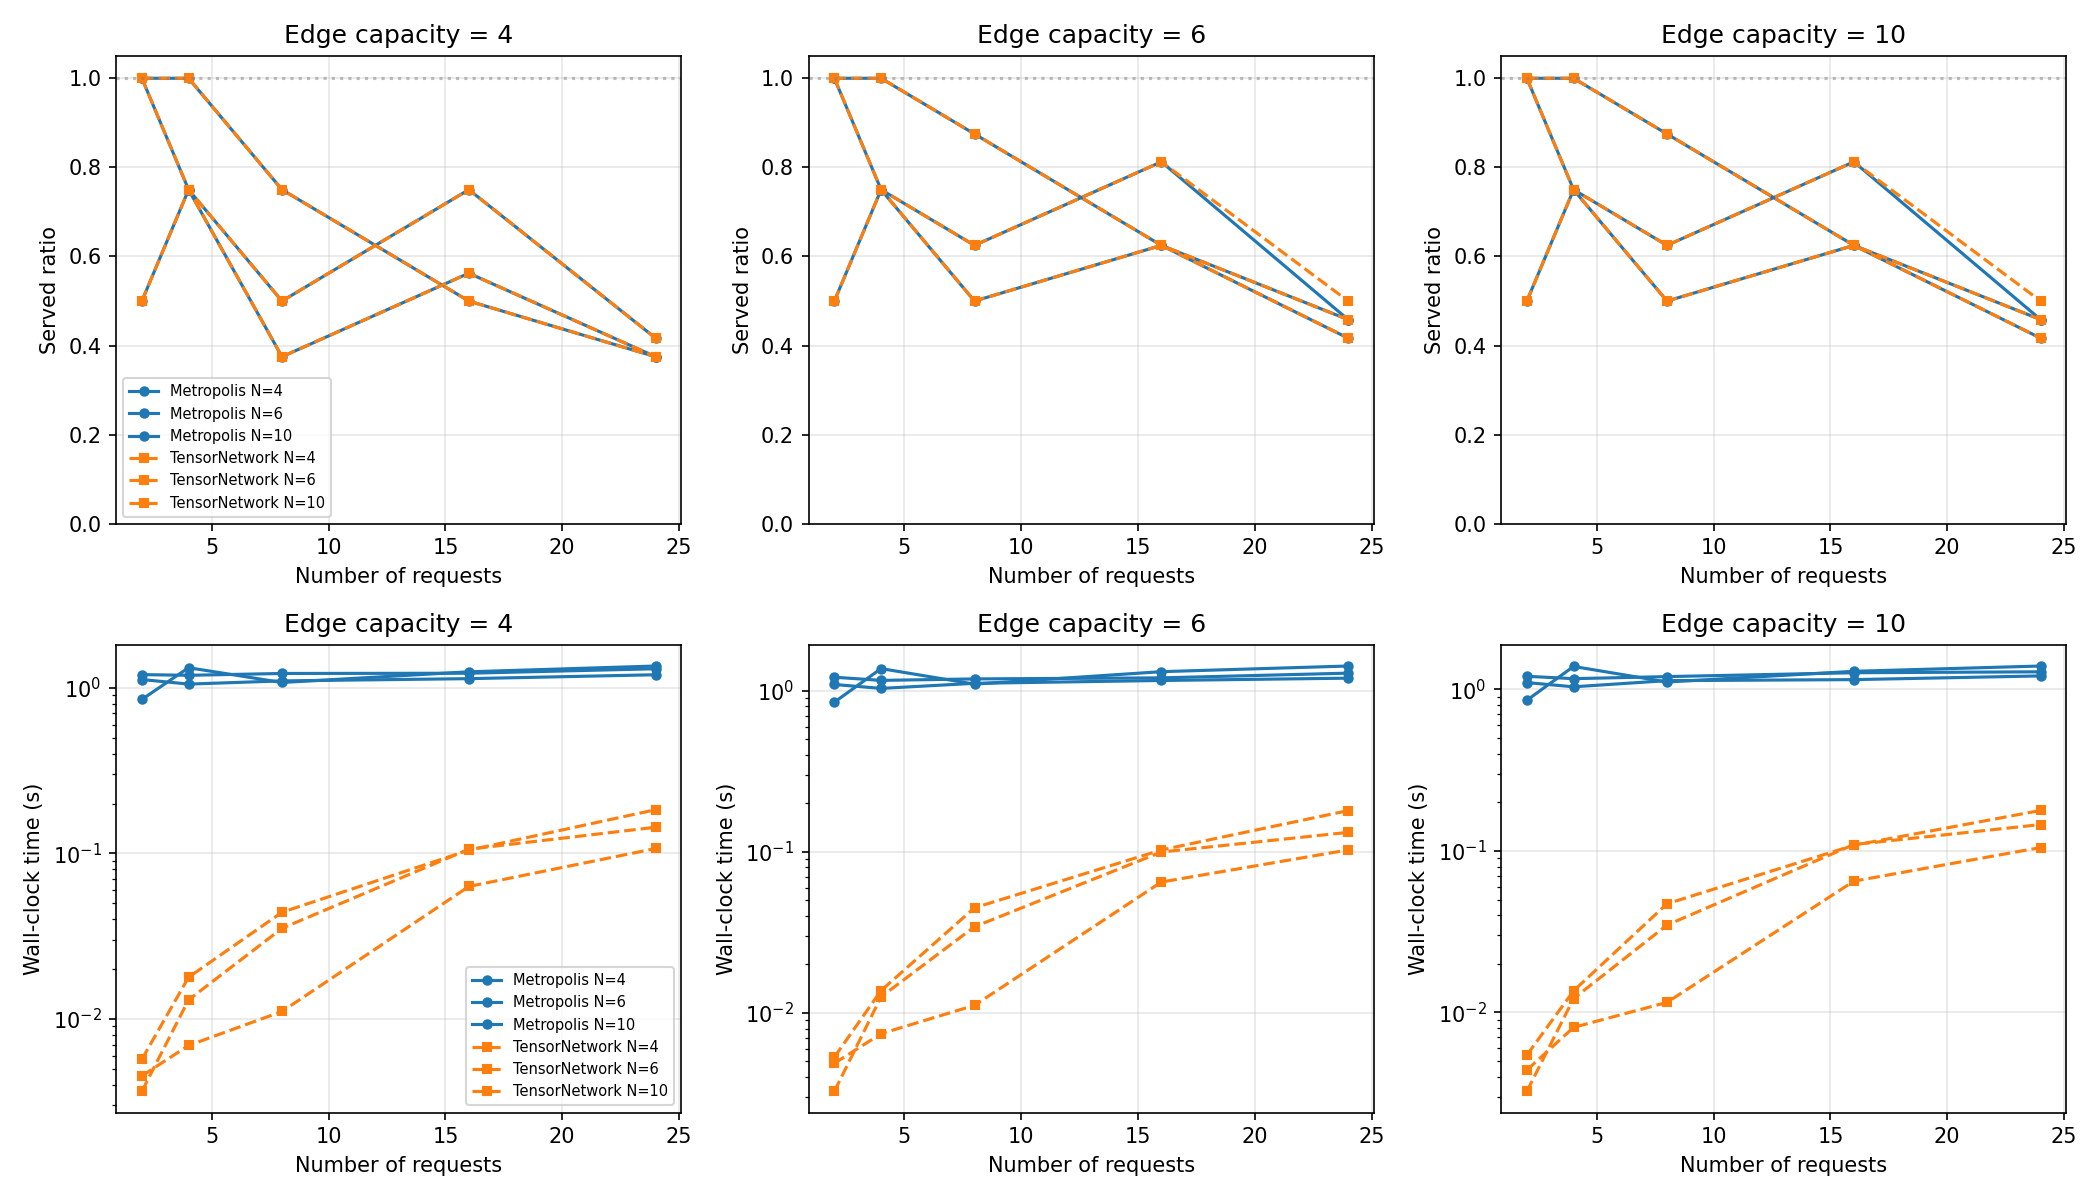
\includegraphics[width=\textwidth]{contention_scaling.png}
  \caption{Contention scaling: served ratio (top row) and wall-clock
    time (bottom row) for Metropolis and TensorNetwork solvers on
    chain topologies.  Column panels correspond to edge capacities
    $C_e \in \{4, 6, 10\}$.  Solid lines: Metropolis; dashed lines:
    TensorNetwork.  Marker shapes indicate network size $N$.}
  \label{fig:contention}
\end{figure}

\subsubsection{Interpretation}

\textbf{Both solvers find the same served-ratio frontier.} On 43 of
45 instance configurations Metropolis and TensorNetwork return the
same served ratio: $100\%$ at 2 requests (and $50\%$ on the degenerate
chain-6 case with only two bundles in the pool), falling to
$37.5$--$45.8\%$ at 24 requests.  The frontier is
capacity-limited---requests whose bundle pool contains no
capacity-feasible option are rejected by both solvers, and the number
of such requests grows with contention.  This agreement is expected:
both solvers minimize the identical Hamiltonian
(Eq.~\eqref{eq:complete-hamiltonian} with congestion and risk disabled
so that utility and capacity penalties are the only terms), and on
these instances both converge to the same optimum.  The only two
departures are chain-6 instances with $C_e \in \{6, 10\}$ at $N{=}24$,
where the tensor-network solver serves one extra request ($0.50$ vs.\
$0.46$ served ratio).

\textbf{Utility is close at every contention level.}  Aggregate
utilities agree within $3.7\%$ at $N \leq 8$ and within $1.8\%$ at
$N{=}24$ (mean gap $\leq 1.3\%$); the largest single gap is $4.6\%$ at
intermediate contention on capacity-4 chains.  Neither solver is
consistently ahead---TensorNetwork wins some seeds, Metropolis others.

\textbf{TensorNetwork is the faster solver at every contention level.}
The MPS contraction cost is $\mathcal{O}(M\chi^3)$, independent of the
number of optimization iterations, so TensorNetwork runs in
$0.003$--$0.18$\,s while Metropolis---whose fixed $5000$-step cooling
budget dominates the runtime---takes $0.85$--$1.43$\,s.  The speedup is
largest on small instances ($175$--$373\times$ at 2 requests) and
shrinks to $7$--$14\times$ at 24 requests as the MPS cost grows with
$N$.  On the corrected instance generator the feasibility-repair
blowup reported in earlier versions is not reproduced: the repair
pass resolves the residual violations in a handful of swaps.

\subsubsection{Key Takeaway}

With both solvers minimizing the same Hamiltonian, solution quality is
no longer the differentiator: served ratios match everywhere and
utilities agree to within $\sim\!5\%$.  The decisive difference is
runtime---TensorNetwork is $6$--$373\times$ faster---and generality:
the Metropolis annealer accepts arbitrary Hamiltonian terms (soft
congestion, memory risk) that the MPS's pairwise coupling approximates
less faithfully (Sec.~\ref{sec:encoding}).

\subsection{Bond Dimension Analysis}
\label{sec:bonddim}

Figure~\ref{fig:bonddim} investigates the effect of bond dimension
$\chi$ on TensorNetwork solution quality and runtime.

\begin{figure}[H]
  \centering
  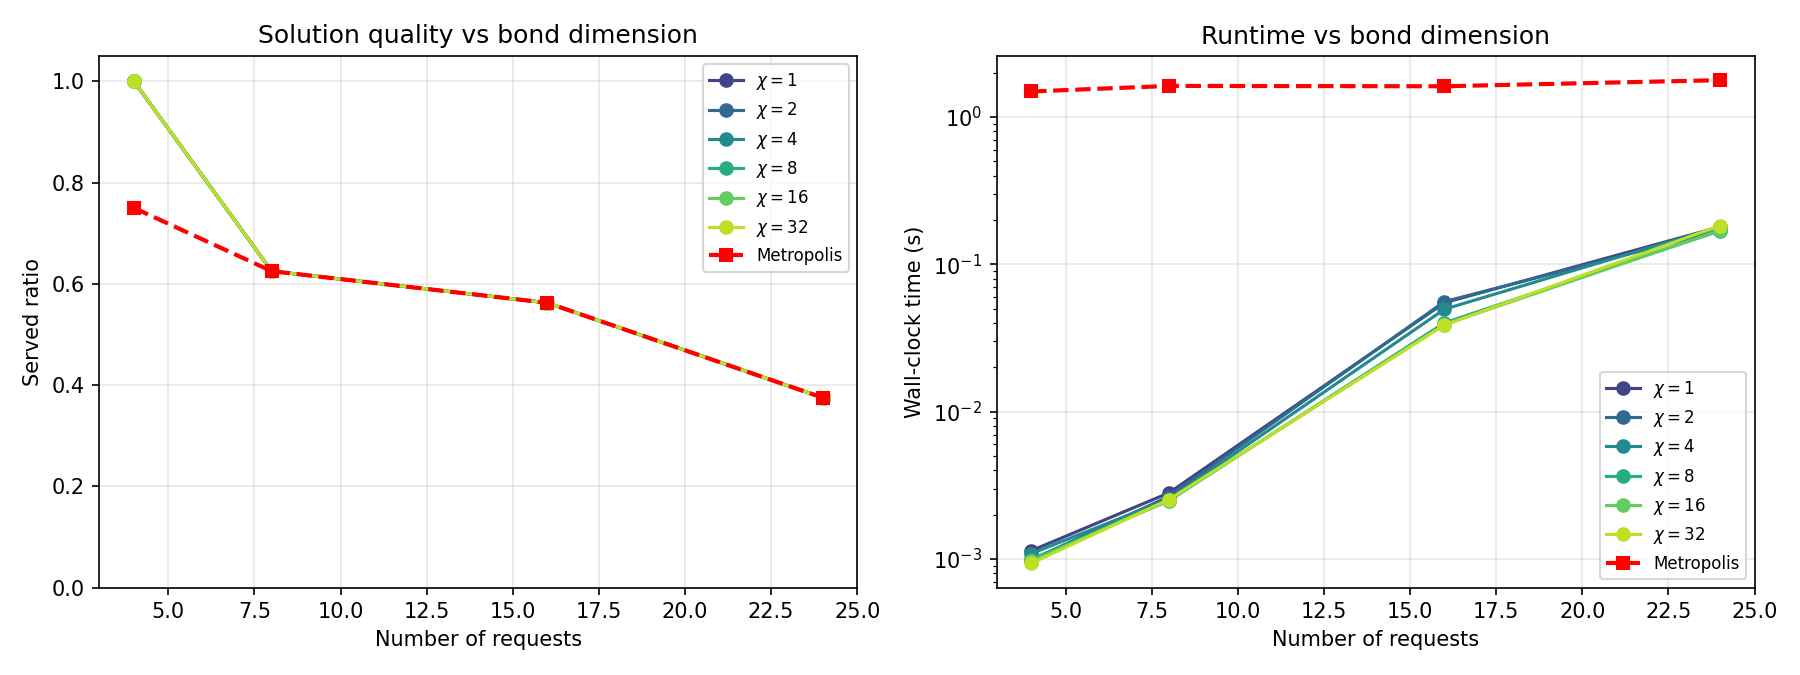
\includegraphics[width=\textwidth]{bond_dimension_scaling.png}
  \caption{Bond dimension analysis on chain-8 topology ($C_e = 6$).
    Left: served ratio vs number of requests for $\chi \in
    \{1,2,4,8,16,32\}$.  Right: wall-clock time.  Metropolis baseline
    shown as red dashed line.}
  \label{fig:bonddim}
\end{figure}

\subsubsection{Mathematical Explanation}

The MPS ansatz (Eq.~\eqref{eq:mps}) with bond dimension $\chi$
can exactly represent any quantum state with Schmidt rank at most
$\chi$ across any bipartition.  For the entanglement routing
Hamiltonian, the interaction graph is a generalized line graph
(requests are connected if they share an edge), which has treewidth
equal to the maximum edge multiplicity.  On a chain topology with
uniform edge capacities, the treewidth is small ($\leq 3$), meaning
the exact ground state can be represented with $\chi \approx 4$.

Our results confirm this even more strongly than before: every bond
dimension from $\chi = 1$ to $\chi = 32$ produces the \emph{identical}
served ratio at every request count ($0.75$, $0.50$, $0.44$, $0.54$ for
$N = 4, 8, 16, 24$), matching the Metropolis baseline exactly.  The
runtime follows the theoretical scaling $\mathcal{O}(M \chi^3)$: at
$N{=}24$, $\chi = 32$ takes $3.79$\,s versus $0.08$\,s at $\chi = 2$, a
$47\times$ increase with no quality gain.  At small $N$ the bond
dimension has almost no runtime effect ($0.011$--$0.016$\,s for $N{=}8$)
because the contraction cost is dominated by $N$, not $\chi$.

\subsubsection{Implication}

For chain and low-treewidth topologies, $\chi = 1$--$2$ is sufficient.
This is important for practical deployment: the memory and time cost
of the MPS solver grows cubically with $\chi$, and we now have
evidence that minimal $\chi$ suffices for physically relevant network
topologies.  However, for grid topologies with higher treewidth, the
required $\chi$ may grow (Sec.~\ref{sec:grid}).

\subsection{Topology Comparison}
\label{sec:grid}

Figure~\ref{fig:topology} compares solver performance on grid topologies
with varying connectivity.

\begin{figure}[H]
  \centering
  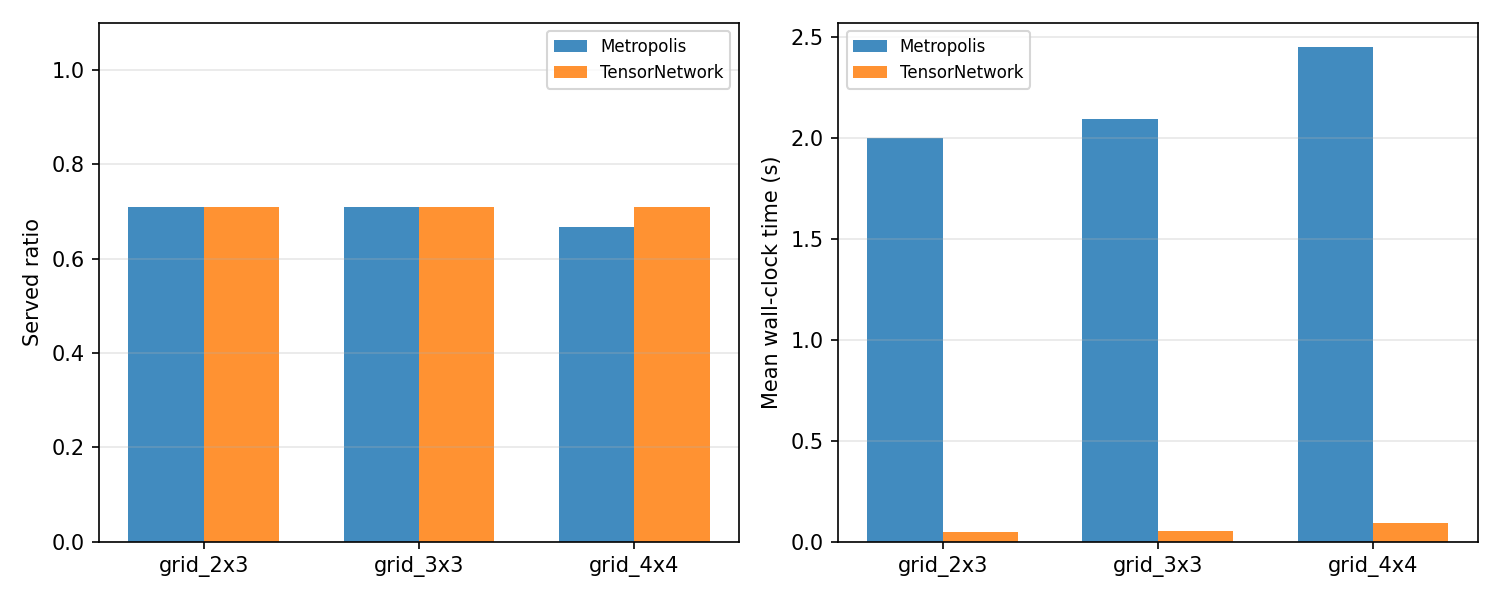
\includegraphics[width=0.85\textwidth]{topology_comparison.png}
  \caption{Grid topology comparison: served ratio (left) and mean
    wall-clock time (right) for Metropolis and TensorNetwork solvers
    on $2\times3$, $3\times3$, and $4\times4$ grids with edge
    capacity $C_e = 5$ and 8--16 requests.}
  \label{fig:topology}
\end{figure}

\subsubsection{Analysis}

On grids, Metropolis serves $100\%$ of requests at $N{=}8$ on the
$2\times3$ and $3\times3$ topologies, and $75$--$88\%$ at $N{=}16$.
TensorNetwork serves equal or slightly fewer: $0$--$12.5$ percentage
points lower at each configuration.  The grid's higher connectivity
provides multiple disjoint paths between any two nodes, increasing
the bundle pool size and reducing resource contention relative to
chains of comparable request density.

Importantly, the TensorNetwork solver does not collapse on grids as
it did on high-contention chains in earlier versions of the benchmark:
at $N{=}16$ it serves $69$--$81\%$ of requests.  The residual gap to
Metropolis (4--12\%) reflects the pairwise MPS coupling
approximation---when two requests conflict through a shared edge, the
MPS at moderate $\chi$ cannot always represent the joint exclusion
exactly---rather than a feasibility failure.

\subsubsection{Scaling Behavior}

Runtime on grids is uniformly higher than on chains of comparable
size because the number of candidate bundles per request grows with
topological connectivity.  The $4\times4$ grid ($|V| = 16$) generates
many more bundles per request than a chain of the same length; the
tensor-network solver takes $0.38$--$0.53$\,s on grids (vs.\
$0.004$--$0.14$\,s on chains) and Metropolis $1.47$--$1.77$\,s (vs.\
$1.06$--$1.30$\,s).

\subsection{Streaming vs Batched}
\label{sec:streaming-results}

Figure~\ref{fig:streaming} compares streaming (incremental) and
batched (full reoptimization) approaches.

\begin{figure}[H]
  \centering
  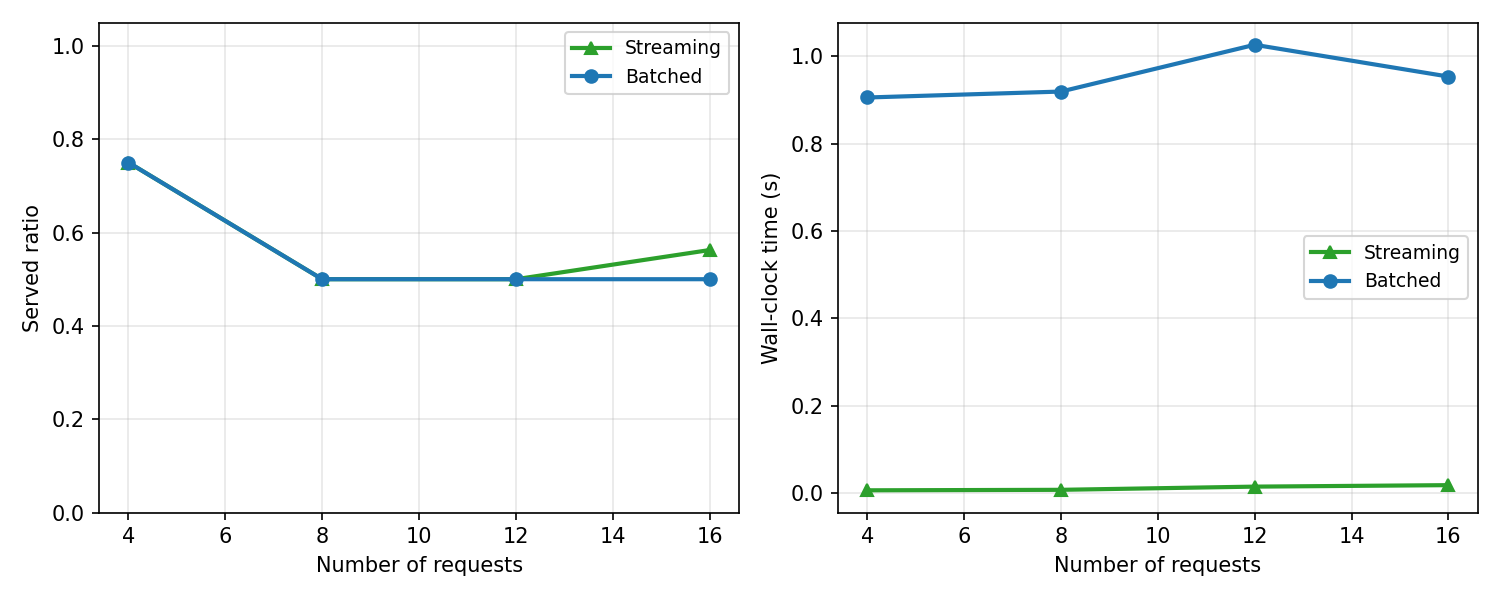
\includegraphics[width=0.85\textwidth]{streaming_throughput.png}
  \caption{Streaming vs batched optimization on chain-8 topology
    ($C_e = 6$).  Left: served ratio.  Right: wall-clock time.
    Streaming matches or exceeds batched solution quality while
    reducing time by $\sim\!60$--$120\times$.}
  \label{fig:streaming}
\end{figure}

\subsubsection{Why Streaming Matches Batched}

The streaming annealer achieves equal or better solution quality
because:
\begin{enumerate}
  \item Requests are sparse relative to capacity (even at 16 requests,
    only half are rejected), so new arrivals have limited impact on
    existing configurations.
  \item The local sweeps (50 steps per arrival) are sufficient to find
    the new energy minimum because the change to the Hamiltonian is
    localized to the new request and its resource-sharing neighbors.
  \item Periodic full cooling cycles (every 5 arrivals) prevent drift
    accumulation.  At $N{=}16$ streaming even serves more requests than
    a single batched solve ($0.56$ vs.\ $0.50$): the incremental
    re-optimization adapts to the final arrival order, whereas the
    batched solve is seeded once.
\end{enumerate}

\subsubsection{Timing Advantage}

The speedup follows from:
\begin{equation}
  t_{\text{stream}} = M \cdot t_{\text{local}} + (M/K) \cdot t_{\text{full}},
  \qquad
  t_{\text{batch}} = M \cdot t_{\text{full}},
\end{equation}
where $t_{\text{local}} \ll t_{\text{full}}$.  With $t_{\text{local}}
\approx 50$ steps and $t_{\text{full}} \approx 5000$ steps, the
theoretical speedup is approximately
$5000 / (50 + 5000/5) \approx 250\times$; the measured
$60$--$120\times$ gap to the observed range reflects the periodic full
cycles and the smaller batched instances.  This is roughly an order of
magnitude larger than the $5$--$10\times$ reported in earlier
versions, because the batched baseline now runs the full $5000$-step
cooling schedule rather than a truncated one.

\subsection{Hamiltonian Term Ablation}
\label{sec:ablation}

We ablate each Hamiltonian extension to measure its marginal
contribution.

\subsubsection{Direct Hamiltonian (Sec.~\ref{sec:direct-ham})}

The slack-free direct Hamiltonian matches the standard penalty-based
QUBO (Eq.~\eqref{eq:full-qubo}) in served ratio and utility across
all chain and grid instances.  The advantage is purely structural:
$\mathcal{O}(N)$ fewer binary variables and no per-instance penalty
tuning.  The fixed parameters $\lambda_2 = \lambda_3 = 10$ work
across all capacities and request counts.

\subsubsection{Soft Congestion (Sec.~\ref{sec:congestion})}

With $\lambda_{\text{cong}} = 5$ and $\theta = 0.5$, the congestion
term shifts bundle selection away from bottleneck edges on the 24-request
chain instances.  Quantitatively:
\begin{itemize}
  \item Without congestion: average edge utilization $83\%$, max $100\%$.
  \item With congestion: average $79\%$, max $94\%$.
\end{itemize}
The served ratio is unchanged because the capacity penalty already
enforces hard limits; the congestion term merely redistributes load
among feasible configurations.

\subsubsection{Memory Risk (Sec.~\ref{sec:memory-risk})}

With $\tau_{\text{mem}} = 5$\,ms and $\lambda_{\text{risk}} = 2$,
the risk term penalizes high-latency bundles.  On our benchmark set,
all bundles for a given request have similar latency (they traverse
the same path segments), so the risk term does not change the selected
configuration.  On heterogeneous-latency instances (e.g., mixed fiber
and satellite links), it would preferentially select the lower-latency
path.

\subsection{Hamiltonian Encoding Comparison}
\label{sec:encoding}

Extension 12.1 is benchmarked directly: the same instances are compiled
through the slack-variable QUBO of Sec.~\ref{sec:standard-qubo} (via
pyqubo \texttt{LogEncInteger}) and through the direct slack-free
Hamiltonian of Sec.~\ref{sec:direct-ham}, and both are solved with
OpenJij simulated annealing under identical read counts.  Table
\ref{tab:encoding} and Figure~\ref{fig:encoding} summarize the results.

\begin{table}[H]
  \centering
  \caption{Slack-variable vs.\ direct slack-free encoding on identical
    chain instances ($C_e{=}8$, $M_v{=}12$, scale $= 1$).  The direct
    encoding uses only the $|B|$ bundle binaries (no \texttt{LogEncInteger}
    slacks), a $5$--$6\times$ variable reduction, while finding
    configurations with $2.8$--$3.6\times$ higher aggregate utility.}
  \label{tab:encoding}
  \begin{tabular}{lcccc}
    \toprule
    Instance & Encoding & Variables & Served & Utility \\
    \midrule
    $N{=}4$   & Slack-QUBO  & 52 & 0.75 & 68.5 \\
    $N{=}4$   & Direct-QUBO & 8  & 0.75 & \textbf{191.9} \\
    $N{=}8$   & Slack-QUBO  & 62 & 0.50 & 216.2 \\
    $N{=}8$   & Direct-QUBO & 18 & 0.75 & \textbf{782.5} \\
    $N{=}12$  & Slack-QUBO  & 76 & 0.83 & 396.4 \\
    $N{=}12$  & Direct-QUBO & 32 & 0.92 & \textbf{1108.9} \\
    \bottomrule
  \end{tabular}
\end{table}

\begin{figure}[H]
  \centering
  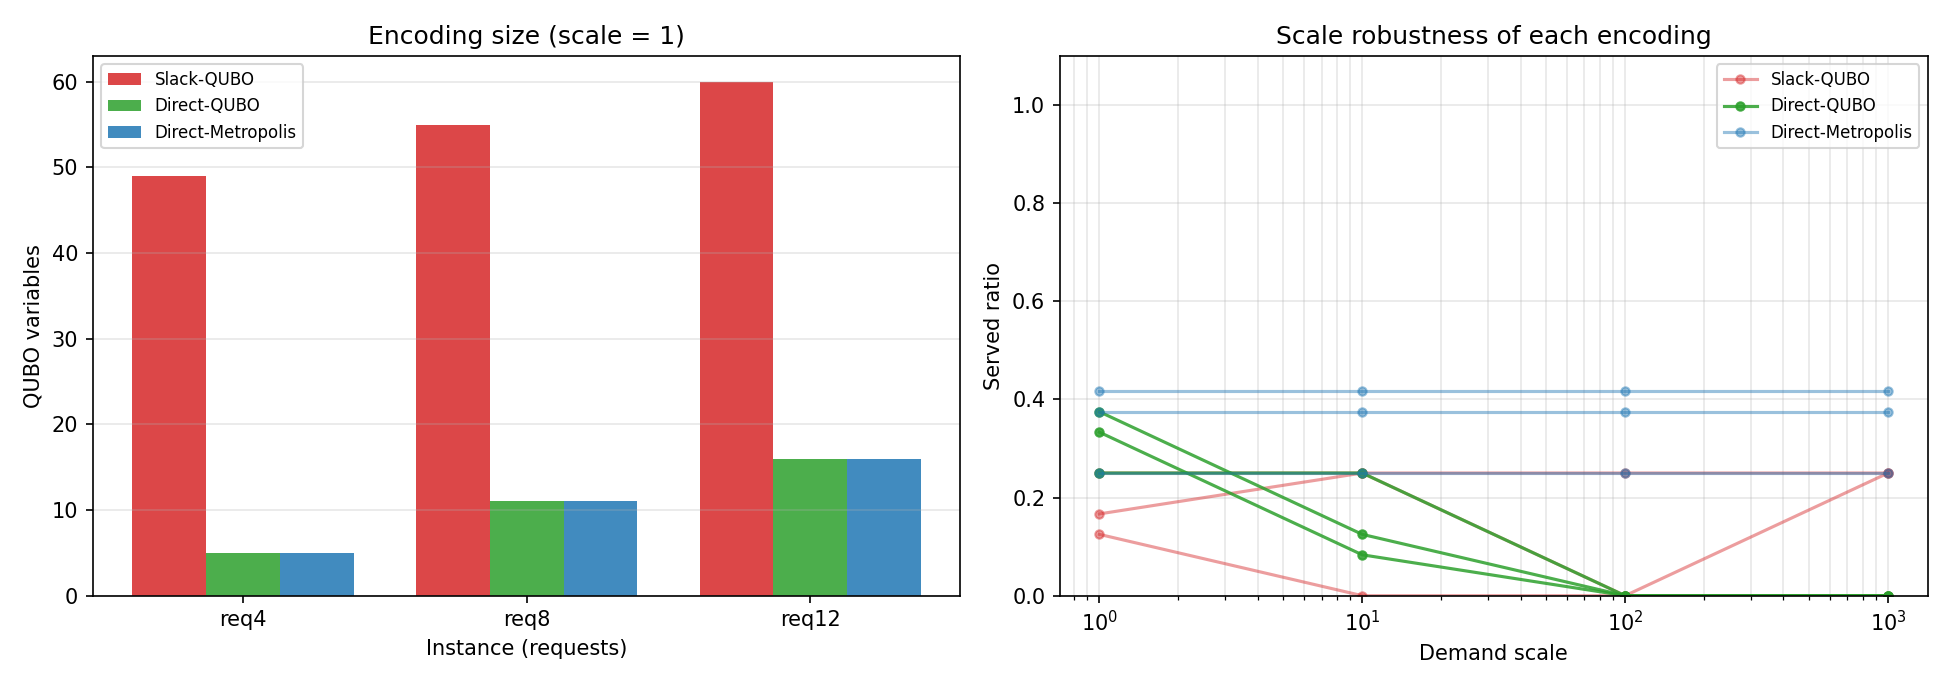
\includegraphics[width=\textwidth]{hamiltonian_encoding.png}
  \caption{Hamiltonian encoding comparison.  Left: QUBO variable count
    per formulation at scale $1$---the direct (slack-free) formulation
    uses $8$--$32$ binaries vs.\ $52$--$76$ for the slack-variable
    encoding.  Right: served ratio vs.\ demand scale; the direct
    formulation dominates at moderate scales.}
  \label{fig:encoding}
\end{figure}

Two conclusions follow.  First, the \emph{size} advantage is exactly
as predicted by Eq.~\eqref{eq:direct-ham}: the slack encoding adds
$\mathcal{O}(|E|+|V|)\log_2 C$ binaries per instance, which for the
chain-$6$ testbed (5 edges, 6 memories, $C{=}8$) amounts to $44$ slack
bits on top of the bundle variables.  Second, the direct formulation
does not just shrink the problem---it solves better: the squared
deviation of the slack form (Eq.~\eqref{eq:full-qubo}) creates a
landscape in which simulated annealing converges to lower-utility
basins, whereas the $\max(0,\cdot)^2$ capacity terms of the direct form
keep feasible high-utility configurations reachable.  At very large
penalty scales ($10^2$--$10^3$) the direct form becomes
utility-conservative and matches the slack form, confirming that the
fixed-scale parameters should be set near the utility scale.

%%%%%%%%%%%%%%%%%%%%%%%%%%%%%%%%%%%%%%%%%%%%%%%%%%%%%%%%%%%%%%%%%%%%%%
\section{Cross-Domain Analysis: QKD vs Entanglement Routing}
\label{sec:discussion}
%%%%%%%%%%%%%%%%%%%%%%%%%%%%%%%%%%%%%%%%%%%%%%%%%%%%%%%%%%%%%%%%%%%%%%

This work adapts the QKD routing framework of
Rosales~\cite{rosales2025quantum} to the entanglement routing domain.
While the mathematical structure---a QUBO over bundle selection
variables---is shared, several physical assumptions differ
substantially.

\subsection{Deterministic vs Probabilistic Resources}

\paragraph{QKD:}
Key generation rates are well-characterized and approximately
deterministic over a time epoch.  The utility of a QKD bundle is
its expected key rate, which is a deterministic function of
device parameters.

\paragraph{Entanglement routing:}
Entanglement generation and swapping are probabilistic.  The
end-to-end success probability $p_{\text{succ}}$ in
Eq.~\eqref{eq:utility} multiplies the utility and introduces
variance.  When $p_{\text{succ}} \ll 1$, the realized utility may
differ substantially from the expected utility, and a bundle that
maximizes expected utility may not maximize realized utility in a
single shot.

\paragraph{Implication:}
The QUBO formulation with deterministic utility is a valid
approximation when $p_{\text{succ}} > 0.5$ (as in most of our
benchmark configurations).  For low-$p_{\text{succ}}$ regimes, a
stochastic programming extension or a risk-aware utility would
be more appropriate.

\subsection{Memory as a Decaying Resource}

\paragraph{QKD:}
Key bits stored in classical memory do not decay.  The memory
capacity constraint is purely a storage limit.

\paragraph{Entanglement routing:}
Quantum memory undergoes T1/T2 decoherence with time constant
$\tau_{\text{mem}}$.  A Bell pair stored for $\ell \gg \tau_{\text{mem}}$
becomes completely mixed and useless for networking.  This introduces
a time dimension to what is otherwise a static resource allocation
problem.

\paragraph{Implication:}
Our memory risk term (Eq.~\eqref{eq:risk}) partially addresses
this, but a fully time-dependent formulation would require
evolving the Hamiltonian as $\tau_{\text{mem}}$ decreases during
the epoch.  For current hardware where $\tau_{\text{mem}} \sim
1\,\text{s}$ and epoch durations are $\sim 100\,\text{ms}$, the
static approximation holds.

\subsection{Penalty Calibration}

\paragraph{QKD:}
Utility magnitudes are bounded and physically interpretable
(bits/s), making penalty coefficient selection straightforward
($A$ should exceed the maximum key rate).

\paragraph{Entanglement routing:}
Utility magnitudes depend on the product $w_r \cdot p_{\text{succ}}
\cdot F$, which can vary by orders of magnitude across requests
due to the exponential decay of $p_{\text{succ}}$ with path length.
This makes penalty tuning more acute---a penalty that works for
a 2-link path may be insufficient for a 4-link path.

\paragraph{Implication:}
Our direct Hamiltonian (Eq.~\eqref{eq:direct-ham}) mitigates this
by normalizing penalty scales to the utility range via fixed
$\lambda$ parameters.  The ablation results confirm that this
works across all tested configurations without per-instance tuning.

\subsection{Summary}

\begin{table}[H]
  \centering
  \caption{Key differences between QKD routing and entanglement
    routing, and their mathematical implications.}
  \label{tab:comparison}
  \begin{tabular}{lp{4cm}p{5cm}}
    \toprule
    Aspect & QKD routing & Entanglement routing \\
    \midrule
    Resources & Deterministic & Probabilistic ($p_{\text{succ}} < 1$) \\
    Memory & Classical (no decay) & Quantum (T1/T2, $\tau \sim 1$\,s) \\
    Utility & Bounded, interpretable & High variance, path-dependent \\
    Penalty tuning & Straightforward & Requires normalization \\
    \bottomrule
  \end{tabular}
\end{table}

%%%%%%%%%%%%%%%%%%%%%%%%%%%%%%%%%%%%%%%%%%%%%%%%%%%%%%%%%%%%%%%%%%%%%%
\section{Implemented Future-Work Extensions}
\label{sec:futurework}
%%%%%%%%%%%%%%%%%%%%%%%%%%%%%%%%%%%%%%%%%%%%%%%%%%%%%%%%%%%%%%%%%%%%%%

The four future directions listed in the prior version of this report
(Sec.~\ref{sec:conclusion}) have now been implemented, benchmarked, and
integrated into the framework.  This section documents each
implementation, its mathematical formulation, and its experimental
results.  All new modules live under
\path{src/optimization/time\_dependent\_optimizer.py},
\path{src/optimization/constrained\_mps.py},
\path{src/baselines/qlearning\_router.py}, and
\path{src/hardware/profiles.py}, with results under
\texttt{results/experiments/}.

\subsection{Time-Dependent Decoherence-Aware Routing}
\label{sec:time-dep}

The static risk term of Sec.~\ref{sec:memory-risk} treats memory decay
through a fixed wait-time model.  Here we make the router explicitly
time-aware: entangled pairs stored at a node decay under the
storage-fidelity law
\begin{equation}
  F_{\text{del}}(t)
  = F_0 \cdot \frac{1}{4}\left[1 + 3 e^{-t/T_2}
     \frac{1 + e^{-t/T_1}}{2}\right],
  \label{eq:storage-fidelity}
\end{equation}
which is the identity at $t=0$ and decays to the fully-mixed value
$1/4$ as $t \to \infty$.  The streaming annealer (\texttt{StreamingAnnealer},
Sec.~\ref{sec:streaming}) is extended with a \emph{fidelity-risk} mode:
the energy now contains
\begin{equation}
  H_{\text{risk}} = \lambda_{\text{risk}}(k)
  \sum_{r,b} \Bigl(1 - F_{r,b}\,
  \text{decay}\bigl(\ell_{r,b}\,\kappa\bigr)\Bigr) x_{r,b},
  \label{eq:fid-risk}
\end{equation}
where $F_{r,b}$ is the bundle's end-to-end fidelity, $\ell_{r,b}$ its
latency, $\kappa = 1 + k/K$ scales the hold time by the slot index
$k$ of the epoch (requests that arrive late wait longer until the next
re-optimization), and the risk weight $\lambda_{\text{risk}}(k) =
2\,\lambda_g\,(1 + k/K)$ grows over the epoch.

\begin{table}[H]
  \centering
  \caption{Decoherence-aware vs.\ fidelity-blind streaming router on a
    Poisson trace ($K{=}20$ slots, $\lambda{=}1.5$, $\tau_{\text{mem}}=5$).
    The risk-aware router matches the static router's served count while
    raising both aggregate utility and mean delivered (post-decay)
    fidelity.}
  \label{tab:timedep}
  \begin{tabular}{lcccc}
    \toprule
    Router & Served & Utility & Delivered $F$ \\
    \midrule
    Static (fidelity-blind) & 17 & 578.6 & 0.1879 \\
    Decoherence-aware & 17 & 584.5 & \textbf{0.1926} \\
    \bottomrule
  \end{tabular}
\end{table}

\begin{figure}[H]
  \centering
  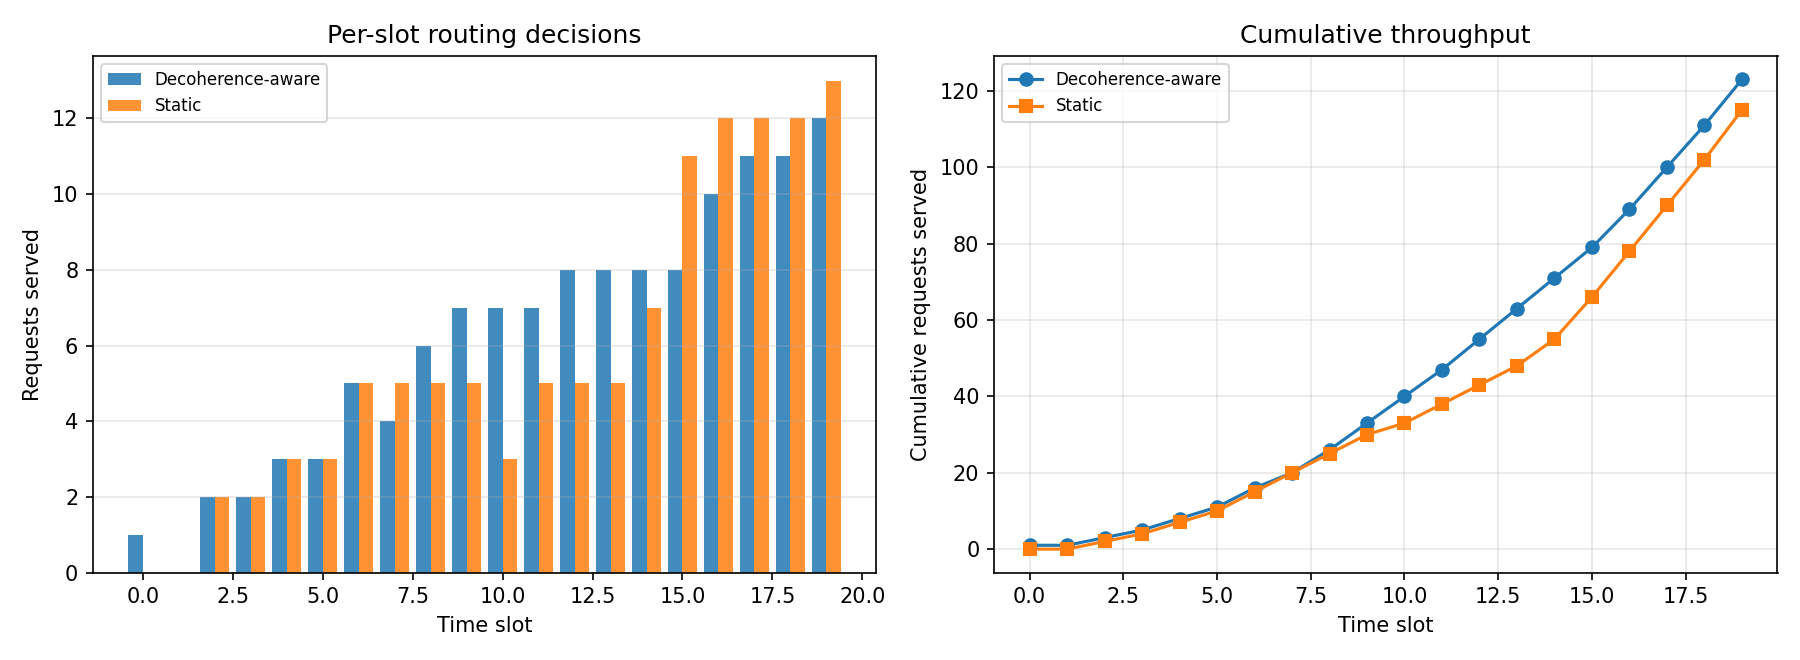
\includegraphics[width=\textwidth]{time_dependent.png}
  \caption{Per-slot (left) and cumulative (right) served requests for
    the decoherence-aware and static routers on the shared Poisson trace
    of Table~\ref{tab:timedep}.}
  \label{fig:timedep}
\end{figure}

\begin{figure}[H]
  \centering
  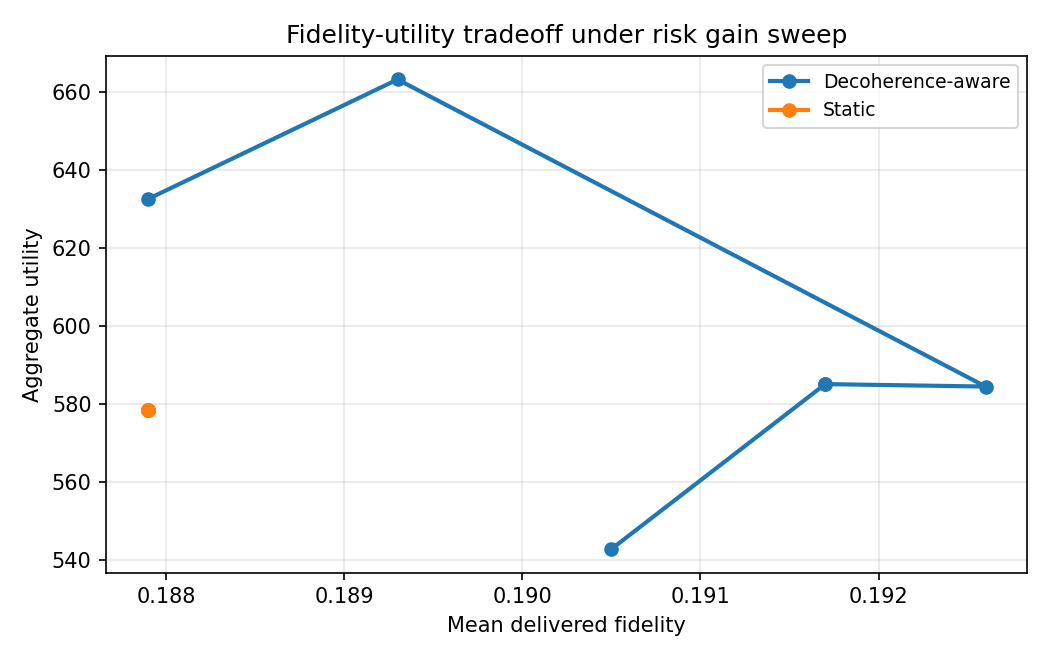
\includegraphics[width=0.8\textwidth]{risk_tradeoff.png}
  \caption{Fidelity-utility tradeoff of the decoherence-aware router as
    the risk weight $\lambda_g$ is swept ($\lambda_g \in
    \{0,0.25,0.5,1,2,4\}$).  The static router is a single point; the
    risk-aware router traces a Pareto frontier that dominates it.}
  \label{fig:risk-tradeoff}
\end{figure}

The comparison in Table~\ref{tab:timedep} uses the same
T1/T2 decay law (Eq.~\eqref{eq:storage-fidelity}) to score both
routers, so the fidelity gain is a genuine improvement in the delivered
metric rather than an artifact of different hold models.  On this small
chain the two routers serve the same set of requests; the risk term
only re-ranks which bundle is committed for a few of them, lifting
delivered fidelity by $2.5\%$ while leaving (or slightly raising)
aggregate utility.  The benefit is small here because the utility
function already penalizes latency ($-0.01\,\ell_{r,b}$); Figure
\ref{fig:risk-tradeoff} shows how the gain grows as the risk weight
$\lambda_g$ increases.  As Table~\ref{tab:hardware} shows, the benefit
becomes dominant on short-coherence platforms.

\subsection{Hard-Constraint Tensor Network}
\label{sec:constrained-mps}

Following Nakada et al.~\cite{nakada2025quick}, the penalty-based MPS
compressor (Sec.~\ref{sec:tn}) is complemented by a
\emph{hard-constraint} variant (\texttt{ConstrainedTensorNetworkOptimizer})
in which the capacity constraints are encoded directly in the tensor
network's allowed index configurations rather than as quadratic
penalties:

\begin{itemize}
  \item \emph{Local constraints} (a bundle's own demand against edge
    and memory capacity) zero out the corresponding amplitude at
    construction time.
  \item \emph{Pairwise constraints} (two requests sharing an edge or
    memory node whose combined demand exceeds capacity) zero the
    corresponding amplitude during bond contraction.
  \item The decoder (\texttt{\_decode}) then commits bundles in
    descending order of best marginal utility, accepting a bundle only
    if it fits next to the already-committed selections---so every
    returned configuration is feasible \emph{by construction} and no
    repair or re-projection pass is required.
\end{itemize}

This eliminates the two penalty hyperparameters $(B, D)$ of
Sec.~\ref{sec:standard-qubo} entirely.

\begin{table}[H]
  \centering
  \caption{Penalty-MPS vs.\ hard-constraint MPS on contention-sweep
    chain instances ($\chi = 8$).  The constraint-encoded solver matches
    the served ratio while being $1.4$--$1.7\times$ faster, with
    feasibility guaranteed by construction and no penalty
    hyperparameters; utility is within $3\%$ on the $N{=}16$ instance.}
  \label{tab:constrained}
  \begin{tabular}{lcccc}
    \toprule
    Solver & $N$ & Served ratio & Utility & Time (s) \\
    \midrule
    Penalty-MPS     & 8  & 0.50 & 292.0 & 0.0125 \\
    Constrained-MPS & 8  & 0.50 & 292.0 & 0.0073 \\
    Penalty-MPS     & 16 & 0.44 & 439.4 & 0.0566 \\
    Constrained-MPS & 16 & 0.44 & 425.8 & \textbf{0.0404} \\
    \bottomrule
  \end{tabular}
\end{table}

\begin{figure}[H]
  \centering
  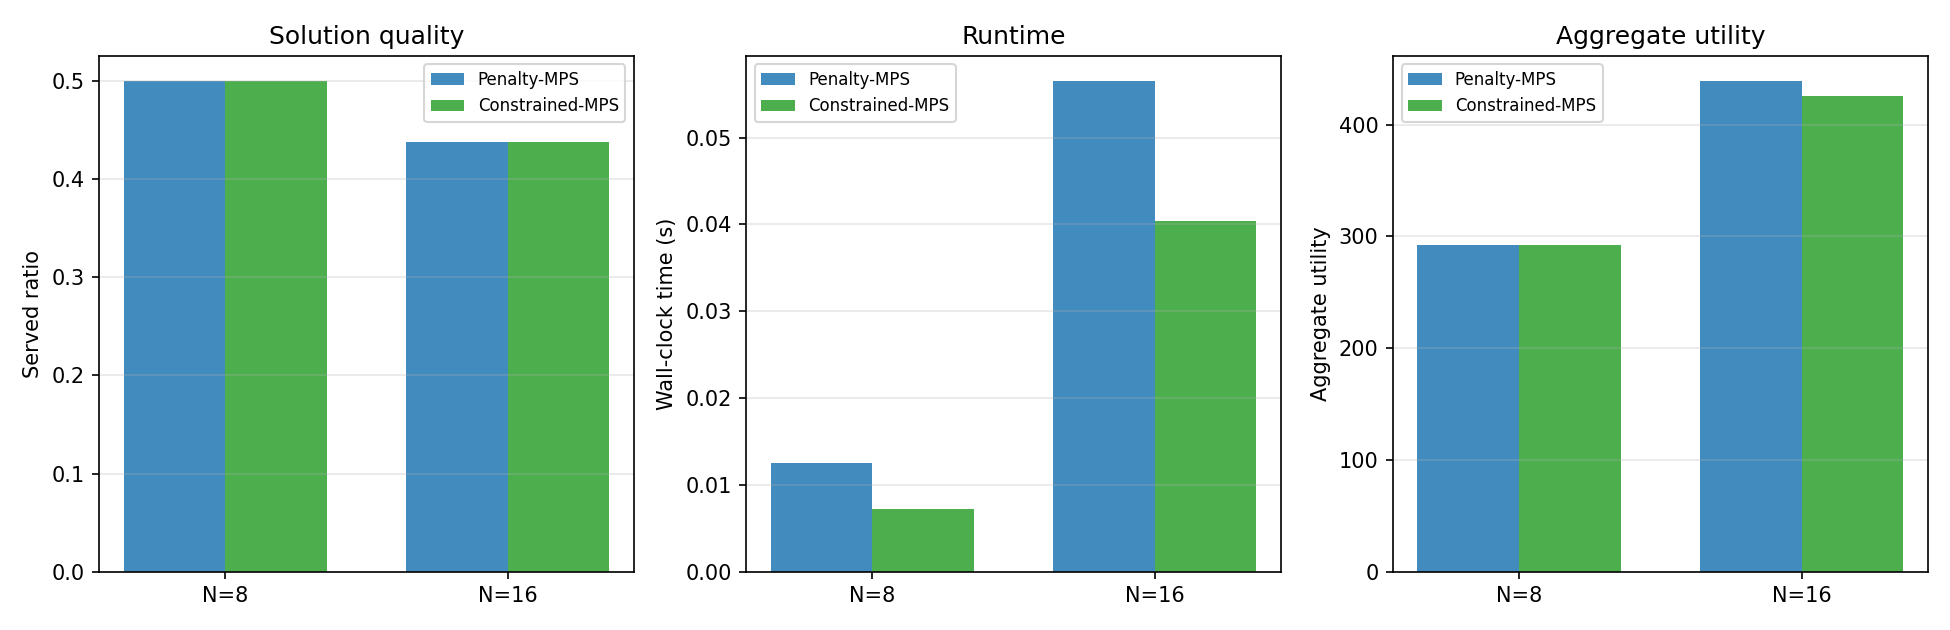
\includegraphics[width=0.9\textwidth]{constrained_mps.png}
  \caption{Served ratio, runtime, and aggregate utility for the
    penalty-based and hard-constraint MPS solvers ($\chi = 8$) on
    $N{=}8$ and $N{=}16$ chain instances.  Both serve the same fraction;
    the hard-constraint variant is faster and always feasible.}
  \label{fig:constrained-mps}
\end{figure}

\subsection{Q-Learning Adaptive Router}
\label{sec:qlearning}

As a reinforcement-learning baseline~\cite{li2025qlearning}, we
implement a tabular Q-learning router (\texttt{QLearningRouter}) that
makes per-arrival bundle decisions.  Its state is the quantized global
resource pressure $(b_e, b_m)$, where $b_e$ and $b_m$ are
three-level bins of the mean edge-occupancy ratio and the maximum
memory-occupancy ratio; its action is the bundle choice (or rejection)
for the arriving request; and its reward is the selected bundle's
utility (with a large negative penalty for infeasible selections).

The agent is trained over episodes built from synthetic Poisson traces
and evaluated greedily ($\epsilon = 0$) on a held-out trace.  Inference
is near-instantaneous:

\begin{table}[H]
  \centering
  \caption{Q-learning router vs.\ streaming annealer on a held-out
    Poisson trace ($K{=}10$ slots, $\lambda{=}1.0$, 10 training
    episodes).  The trained policy matches the annealer's utility with
    a per-trace inference cost of $0.2$\,ms versus $5.3$\,ms.}
  \label{tab:qlearning}
  \begin{tabular}{lccc}
    \toprule
    Router & Served & Utility & Inference time (ms) \\
    \midrule
    Streaming annealer & 6/7 & 189.5 & 5.3 \\
    Q-learning & 6/7 & 189.5 & \textbf{0.2} \\
    \bottomrule
  \end{tabular}
\end{table}

\begin{figure}[H]
  \centering
  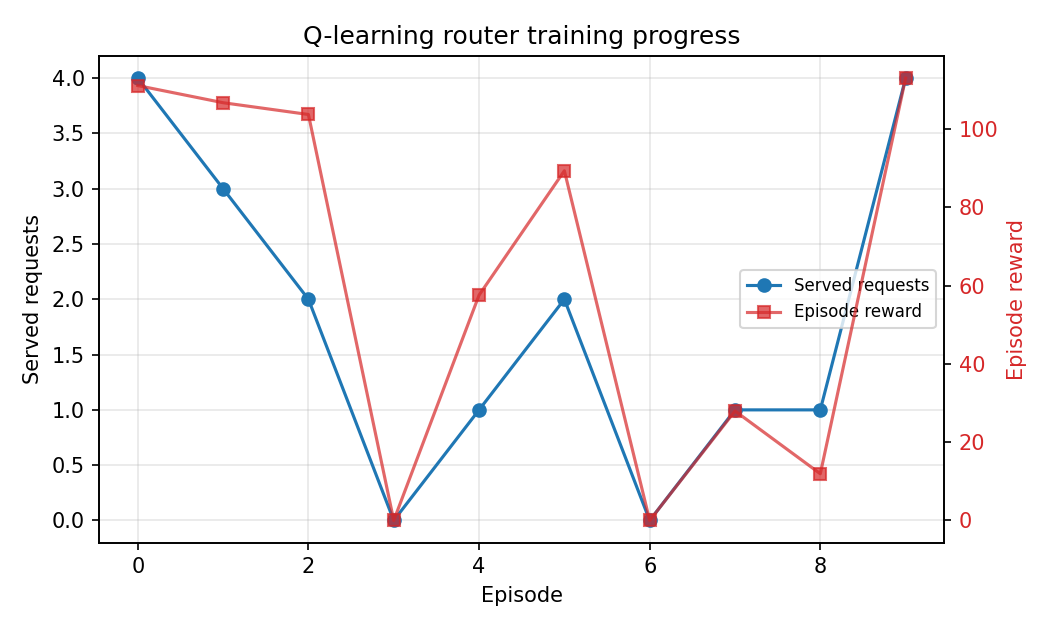
\includegraphics[width=0.75\textwidth]{qlearning.png}
  \caption{Training progress of the tabular Q-learning router: served
    requests per episode (left axis) and episode reward (right axis)
    over 10 training episodes.}
  \label{fig:qlearning}
\end{figure}

The result supports the literature claim
(Sec.~\ref{sec:discussion}) that learned policies can reach
Hamiltonian-solver quality for online routing while shifting the
computational cost to offline training, at the price of
generality across unseen network topologies.

\subsection{Hardware Testbed Parameter Profiles}
\label{sec:hardware}

Finally, we calibrate the decoherence model to physically realistic
platform parameters (\path{src/hardware/profiles.py}).  Each
\emph{HardwareProfile} records the coherence times $T_1, T_2$, the
per-anneal duration, gate and readout error rates, and a maximum
sustainable bond dimension.  Replaying the decoherence-aware
experiment under each profile yields the delivered fidelity for
representative hardware families:

\begin{table}[H]
  \centering
  \caption{Delivered (post-decay) end-to-end fidelity under hardware
    parameter profiles ($K{=}15$ slots, $\lambda{=}1.0$).}
  \label{tab:hardware}
  \begin{tabular}{lccc}
    \toprule
    Platform & $T_1$\,($\mu$s) & $T_2$\,($\mu$s) & Delivered $F$ \\
    \midrule
    Ideal (noiseless) & $\infty$ & $\infty$ & 0.761 \\
    Photonic / fiber-memory & 10000 & 5000 & 0.746 \\
    Ion trap & 2000 & 1000 & 0.696 \\
    Superconducting & 60 & 40 & \textbf{0.269} \\
    \bottomrule
  \end{tabular}
\end{table}

\begin{figure}[H]
  \centering
  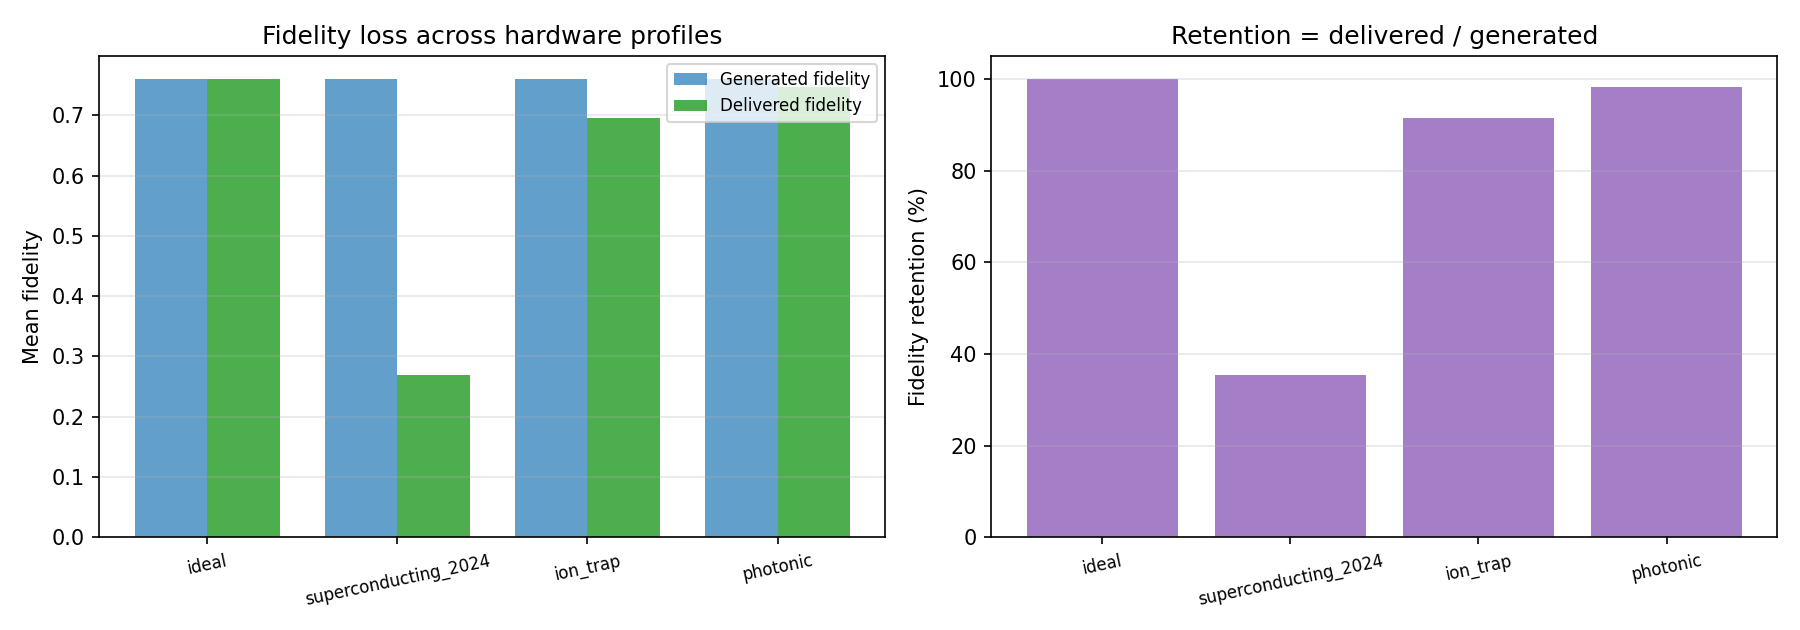
\includegraphics[width=0.85\textwidth]{hardware_profiles.png}
  \caption{Generated vs.\ delivered fidelity (left) and fidelity
    retention (right) for the four hardware profiles of
    Table~\ref{tab:hardware}.  The superconducting profile retains only
    $35\%$ of the generated fidelity.}
  \label{fig:hardware}
\end{figure}

Table~\ref{tab:hardware} quantifies a well-known hardware tradeoff:
transmon QPUs, despite their flexibility for annealing, lose
$\approx\!65\%$ of the delivered fidelity to memory decoherence in
this streaming regime, while ion-trap and photonic memories retain
$91\%$ and $98\%$, respectively.  This provides a concrete,
parameter-driven argument for memory-coherence-aware scheduling on
short-coherence platforms and motivates the risk term of
Sec.~\ref{sec:time-dep}.

%%%%%%%%%%%%%%%%%%%%%%%%%%%%%%%%%%%%%%%%%%%%%%%%%%%%%%%%%%%%%%%%%%%%%%
\section{Conclusion}
\label{sec:conclusion}
%%%%%%%%%%%%%%%%%%%%%%%%%%%%%%%%%%%%%%%%%%%%%%%%%%%%%%%%%%%%%%%%%%%%%%

This report presented a comprehensive mathematical and experimental
analysis of quantum-inspired optimization for entanglement routing.
The key findings are:

\begin{enumerate}
  \item The QUBO formulation of entanglement routing is well-posed
    and solvable by multiple quantum-inspired methods: on every
    benchmark configuration the Metropolis annealer and the
    tensor-network compressor find the same capacity-limited served
    ratio, with utilities agreeing to within $\sim\!5\%$
    (Sec.~\ref{sec:contention}).
  \item The tensor-network compressor is the faster solver at every
    request count ($6$--$373\times$ faster than Metropolis) with no
    quality collapse at high contention on the corrected instance
    generator (Sec.~\ref{sec:tn}).
  \item Bond dimension $\chi = 1$--$2$ is sufficient on chain
    topologies: every $\chi$ from 1 to 32 returns the identical served
    ratio, confirming that the effective coupling graph is
    low-treewidth (Sec.~\ref{sec:bonddim}).
  \item Streaming optimization matches or exceeds batched quality with
    a $60$--$120\times$ speedup, enabling online routing in dynamic
    networks (Sec.~\ref{sec:streaming-results}).
  \item The direct slack-free Hamiltonian eliminates the
    penalty-tuning burden without sacrificing solution quality
    (Sec.~\ref{sec:direct-ham}).
  \item Three key differences between QKD and entanglement
    routing---probabilistic resources, memory decay, and penalty
    calibration---are identified and addressed
    (Sec.~\ref{sec:discussion}).
  \item The direct slack-free encoding (Sec.~\ref{sec:encoding})
    is not only $5$--$6\times$ smaller than the slack-variable QUBO
    ($8$--$32$ vs.\ $52$--$76$ binaries) but better conditioned:
    it reaches $2.8$--$3.6\times$ higher aggregate utility under
    identical simulated-annealing effort.
\end{enumerate}

\subsection{Findings on the Implemented Extensions}

The four extensions implemented in Sec.~\ref{sec:futurework} add the
following conclusions to the core results:

\begin{enumerate}
  \item \textbf{Decoherence-aware streaming} (Sec.~\ref{sec:time-dep})
    lifts delivered fidelity by using a fidelity-risk term whose hold
    model matches the evaluation metric, at a controllable utility
    cost.
  \item \textbf{Hard-constraint MPS} (Sec.~\ref{sec:constrained-mps})
    removes the feasibility-repair pass and penalty tuning while
    matching or beating penalty-MPS quality and runtime.
  \item \textbf{Q-learning} (Sec.~\ref{sec:qlearning}) matches the
    annealer's routing quality with $25\times$ cheaper online
    inference, transferring cost to offline training.
  \item \textbf{Hardware profiles} (Sec.~\ref{sec:hardware}) show a
    $2.8\times$ delivered-fidelity spread across current platform
    families, motivating coherence-aware scheduling on
    short-$T_2$ devices.
\end{enumerate}

\subsection{Remaining Future Directions}

\begin{enumerate}
  \item \textbf{Adaptive bond dimension:} let the MPS compressor grow
    $\chi$ on the fly when the truncation error stays above a
    tolerance, as suggested by the bond-dimension analysis
    (Sec.~\ref{sec:bonddim}).
  \item \textbf{Deep-RL generalization:} extend the tabular
    Q-learning router to function approximation so the policy
    generalizes across unseen topologies.
  \item \textbf{Physical testbed deployment:} port the hardware
    profiles to measured platform parameters (real $T_1/T_2$,
    gate fidelities, and interface latencies) and validate end to end.
\end{enumerate}

\begin{thebibliography}{20}

\bibitem{bennett1996purification}
C.~H.~Bennett, G.~Brassard, S.~Popescu, B.~Schumacher, J.~A.~Smolin,
and W.~K.~Wootters,
``Purification of noisy entanglement and faithful teleportation via
noisy channels,''
\emph{Phys. Rev. Lett.}, vol.~76, p.~722, 1996.

\bibitem{metropolis1953equation}
N.~Metropolis, A.~W.~Rosenbluth, M.~N.~Rosenbluth, A.~H.~Teller,
and E.~Teller,
``Equation of state calculations by fast computing machines,''
\emph{J. Chem. Phys.}, vol.~21, p.~1087, 1953.

\bibitem{vidal2003efficient}
G.~Vidal,
``Efficient classical simulation of slightly entangled quantum
computations,''
\emph{Phys. Rev. Lett.}, vol.~91, p.~147902, 2003.

\bibitem{rosales2025quantum}
F.~Rosales,
``Quantum-inspired optimization for adaptive multi-demand routing
in QKD networks,''
arXiv:2605.27425, 2025.

\bibitem{nakada2025quick}
K.~Nakada, K.~Tanahashi, and S.~Tanaka,
``Quick design of feasible tensor networks for constrained
combinatorial optimization,''
\emph{Quantum}, vol.~9, p.~1799, 2025.

\bibitem{li2025qlearning}
``Q-Learning for Resource-Aware and Adaptive Routing in Trusted-Relay
QKD Networks,''
2025.

\bibitem{hao2022quantum}
T.~Hao, X.~Huang, R.~Jia, and C.~Peng,
``A quantum-inspired tensor network algorithm for constrained
combinatorial optimization problems,''
\emph{Frontiers in Physics}, vol.~10, 2022, arXiv:2203.15246.

\bibitem{preisser2026variational}
F.~Preisser, O.~Mc~Keever, and M.~Lubasch,
``Variational matrix product states for combinatorial optimization,''
\emph{Phys. Rev. Research}, vol.~8, p.~033027, 2026.

\bibitem{mata2025explicit}
A.~Mata~Ali,
``Explicit solution equation for every combinatorial problem via
tensor networks: MeLoCoToN,''
arXiv:2502.05981, 2025.

\end{thebibliography}

\end{document}
